% Author: Izaak Neutelings (October 2021)
% Inspiration
%   "Very special relativity - An illustrated guide", Sander Bais (2007)
%   http://people.uncw.edu/hermanr/GR/Minkowski/Minkowski.pdf
\documentclass[border=3pt,tikz]{standalone}
\usepackage{amsmath} % for \text
\usepackage{etoolbox} % ifthen
\usepackage[outline]{contour} % glow around text
\usetikzlibrary{calc} % for adding up coordinates
\usetikzlibrary{decorations.markings,decorations.pathmorphing}
\usetikzlibrary{angles,quotes} % for pic (angle labels)
\usetikzlibrary{arrows.meta} % for arrow size
\usepackage{xfp} % higher precision (16 digits?)
\contourlength{1.1pt}

\tikzset{>=latex} % for LaTeX arrow head
\colorlet{myred}{red!85!black}
\colorlet{mydarkred}{red!55!black}
\colorlet{mylightred}{red!85!black!12}
\colorlet{myfieldred}{mydarkred!5} % for S' background
\colorlet{myredhighlight}{myred!20} % highlights simultaneity in ladder paradox
\colorlet{myblue}{blue!80!black}
\colorlet{mydarkblue}{blue!50!black}
\colorlet{mylightblue}{blue!50!black!30}
\colorlet{mylightblue2}{myblue!10}
\colorlet{mygreen}{green!80!black}
\colorlet{mypurple}{blue!40!red!80!black}
\colorlet{mydarkgreen}{green!50!black}
\colorlet{mydarkpurple}{blue!40!red!50!black}
\colorlet{myorange}{orange!40!yellow!95!black}
\colorlet{mydarkorange}{orange!40!yellow!85!black}
\colorlet{mybrown}{brown!20!orange!90!black}
\colorlet{mydarkbrown}{brown!20!orange!55!black}
\colorlet{mypurplehighlight}{mydarkpurple!20} % highlights simultaneity in ladder paradox
\tikzstyle{world line}=[myblue!40,line width=0.3]
\tikzstyle{world line t}=[mypurple!50!myblue!40,line width=0.3]
\tikzstyle{world line'}=[mydarkred!40,line width=0.3]
\tikzstyle{mysmallarr}=[-{Latex[length=3,width=2]},thin]
\tikzstyle{mydashed}=[dash pattern=on 3 off 3]
\tikzstyle{rod}=[mydarkbrown,draw=mydarkbrown,double=mybrown,double distance=2pt,
                 line width=0.2,line cap=round,shorten >=1pt,shorten <=1pt]
%\tikzstyle{rod'}=[rod,draw=mydarkbrown!80!red!85,double=mybrown!80!red!85]
\tikzstyle{vector}=[->,line width=1,line cap=round]
\tikzstyle{vector'}=[vector,shorten >=1.2]
\tikzstyle{particle}=[mygreen,line width=0.9]
\tikzstyle{photon}=[-{Latex[length=5,width=4]},myorange,line width=0.8,decorate,
                    decoration={snake,amplitude=1.0,segment length=5,post length=5}]

\def\tick#1#2{\draw[thick] (#1) ++ (#2:0.06) --++ (#2-180:0.12)}
\def\tickp#1#2{\draw[thick,mydarkred] (#1) ++ (#2:0.06) --++ (#2-180:0.12)}
\def\Nsamples{100} % number samples in plot

\begin{document}
  \def\ymin{0.2}
  \def\xmin{1.6}
  \def\xmax{2}
  \def\Nlines{4} % number of world lines (at constant x/t)
  \pgfmathsetmacro\d{0.9*\xmax/\Nlines} % grid size
  \pgfmathsetmacro\D{2*\d} 

% % SPACETIME DIAGRAM
% \begin{tikzpicture}[scale=1.8]
%   \message{Basic spacetime diagram^^J}
  
%   \def\xmax{2}
%   \def\Nlines{4} % number of world lines (at constant x/t)
  
%   % WORLD LINES GRID
%   \message{  Making world lines...^^J}
%   \foreach \i [evaluate={\x=\i*0.9*\xmax/\Nlines;}] in {1,...,\Nlines}{
%     \message{  Running i/N=\i/\Nlines, x=\x...^^J}
%     \draw[world line]   (-\x,-\xmax) -- (-\x,\xmax);
%     \draw[world line]   ( \x,-\xmax) -- ( \x,\xmax);
%     \draw[world line t] (-\xmax,-\x) -- (\xmax,-\x);
%     \draw[world line t] (-\xmax, \x) -- (\xmax, \x);
%   }
  
%   % AXES
%   \draw[->,thick] (0,-\xmax) -- (0,\xmax+0.2) node[left=-1] {$ct$};
%   \draw[->,thick] (-\xmax,0) -- (\xmax+0.2,0) node[below=0] {$x$};
  
% \end{tikzpicture}

% % SPACETIME DIAGRAM with WORLD LINES
% \begin{tikzpicture}[scale=2.0]
%   \message{Worldlines^^J}
  
%   \def\ymin{0.2}
%   \def\xmin{1.6}
%   \def\xmax{2}
%   \def\Nlines{4} % number of world lines (at constant x/t)
%   \pgfmathsetmacro\d{0.9*\xmax/\Nlines} % grid size
%   \coordinate (O) at (0,0);
%   \coordinate (T) at (0,\xmax+0.2);
  
%   % WORLD LINES GRID
%   \message{  Making world lines...^^J}
%   \foreach \i [evaluate={\x=\i*\d;}] in {1,...,\Nlines}{
%     \message{  Running i/N=\i/\Nlines, x=\x...^^J}
%     \draw[world line]   ( \x,-\ymin) -- ( \x,\xmax);
%     \draw[world line t] (-\xmin, \x) -- (\xmax, \x);
%   }
%   \draw[world line] (-\d,-\ymin) -- (-\d,\xmax);
%   \draw[world line] (-2*\d,-\ymin) -- (-2*\d,\xmax);
%   \draw[world line] (-3*\d,-\ymin) -- (-3*\d,\xmax);
  
%   % AXES
%   \draw[->,thick] (0,-\ymin) -- (T) node[left=-1] {$ct$};
%   \draw[->,thick] (-\xmin,0) -- (\xmax+0.2,0) node[below=0] {$x$};
  
%   % VECTORS
%   \draw[vector,myorange] (O) -- (135:0.78*\xmax)
%     node[mydarkorange,left=6,above=-3] {\contour{white}{$x(t)=-ct$}};
%   \draw[vector,myblue] (O) -- ({atan(1/2)}:1.12*\xmax) %(45/2:\xmax)
%     node[mydarkblue,anchor=-155,outer sep=-1] {$x(t)=2ct$};
%   \draw[vector,myorange] (O) -- (45:1.08*\xmax)
%     node[mydarkorange,left=1,above right=-2] {\contour{white}{$x(t)=ct$}};
%   \draw[vector,mypurple] (O) -- (55:1.2*\xmax)
%     node[mydarkpurple,right=10,above] {\contour{white}{$x(t)=vt$}};
%   \draw[vector,mygreen]
%     (-0.10*\xmax,-0.12*\xmax) to[out=35,in=-100] (O)
%     to[out=80,in=-80,looseness=1.5] (0.3*\xmax,1.05*\xmax)
%     node[mydarkgreen,above=-3] {\contour{white}{$x(t)=v(t)t$}};
%   \draw[vector,myred] (O) -- (0,0.88*\xmax)
%     node[mydarkred,below left=0] {\contour{white}{$x(t)=0$}};
%   %\node[right=8,above,mydarkpurple] at (T) {$x(t)=0$};
  
% \end{tikzpicture}


% % SPACETIME DIAGRAM with TWO OBSERVERS
% \begin{tikzpicture}[scale=2.0]
%   \message{Two observers^^J}
  
%   \def\xmin{0.2}
%   \def\xmax{2}
%   \def\R{2.03} % vector length
%   \def\Nlines{4} % number of world lines (at constant x/t)
%   \pgfmathsetmacro\d{0.9*\xmax/\Nlines} % grid size
%   \pgfmathsetmacro\D{2*\d} % distance between observers
%   \coordinate (A) at (0,0); % observer A at t=0
%   \coordinate (B) at (\D,0); % observer B at t=0
%   \coordinate (C) at (2*\d,2*\d); % point of reflection
%   \coordinate (T1) at (0,2*\d); % time of reflection
%   \coordinate (T2) at (0,4*\d); % light returning at x=0
  
%   % WORLD LINES GRID
%   \message{  Making world lines...^^J}
%   \foreach \i [evaluate={\x=\i*\d;}] in {1,...,\Nlines}{
%     \message{  Running i/N=\i/\Nlines, x=\x...^^J}
%     \draw[world line]   ( \x,-\xmin) -- ( \x,\xmax);
%     \draw[world line t] (-\xmin, \x) -- (\xmax, \x);
%   }
  
%   % AXES
%   \draw[->,thick] (0,-\xmin) -- (0,\xmax+0.2) node[above left=-2] {$ct$};
%   \draw[->,thick] (-\xmin,0) -- (\xmax+0.2,0) node[below=0] {$x$};
%   \draw[thick,mydarkred,dashed] (T1) -- (C);
%   \draw[thick,mydarkred,dashed] (T2) -- (2*\d,4*\d);
  
%   % VECTORS
%   \draw[vector,myred] (A) --++ (0,\R)
%     node[mydarkred,above=-2,left=-1] {\contour{white}{$x_\mathrm{A}=0$}};
%   \draw[vector,mygreen] (B) --++ (0,\R)
%     node[mydarkgreen,left=1,above=-4] {\contour{white}{$x_\mathrm{B}'=d$}};
%   \draw[photon,shorten >=1] (C) -- (T2);
%   \fill[mydarkorange] (C) circle(0.04);
%   \draw[photon,shorten >=2] (A) -- (C);
%   \fill[mydarkred] (A) circle(0.04) node[below left=-1] {A}; % observer A
%   \fill[mydarkgreen] (B) circle(0.04) node[fill=white,inner sep=0.5,below=2.5] {B}; % observer B
  
%   % TICKS
%   \node[fill=white,inner sep=1,left=3] at (T1) {$\dfrac{ct_2}{2}=ct_1$};
%   \node[fill=white,inner sep=1,left=3] at (T2) {$ct_2$};
%   \tick{T1}{0};
%   \tick{T2}{0};
  
% \end{tikzpicture}


% % SPACETIME DIAGRAM with TWO MOVING OBSERVERS to show simultaneity
% \begin{tikzpicture}[scale=2.0]
%   \message{Two moving observers^^J}
  
%   \def\xmin{0.2}
%   \def\xmax{2}
%   \def\R{2.3} % vector length
%   \def\Nlines{4} % number of world lines (at constant x/t)
%   \pgfmathsetmacro\ang{73} % angle between ct and ct' axes
%   \pgfmathsetmacro\d{0.9*\xmax/\Nlines} % grid size
%   \pgfmathsetmacro\D{2*\d} % distance between observers
%   \coordinate (A) at (0,0); % observer A at t=0
%   \coordinate (B) at (\D,0); % observer B at t=0
%   \coordinate (C) at (45:{\D*sqrt(2)/(1-cot(\ang))}); % point of reflection
%   %\coordinate (T1) at (\ang:{2*\d/sin(\ang)/sqrt(1-cot(\ang)^2)}); % time of reflection
%   \coordinate (T1) at (\ang:{\D*sqrt(cot(\ang)^2+1)/(1-cot(\ang)^2)}); % time of reflection
%   \coordinate (T2) at (\ang:{2*\D*sqrt(cot(\ang)^2+1)/(1-cot(\ang)^2)}); % time of reflection
  
%   % WORLD LINES GRID
%   \message{  Making world lines...^^J}
%   \foreach \i [evaluate={\x=\i*\d;}] in {1,...,\Nlines}{
%     \message{  Running i/N=\i/\Nlines, x=\x...^^J}
%     \draw[world line]   ( \x,-\xmin) -- ( \x,\xmax);
%     \draw[world line t] (-\xmin, \x) -- (\xmax, \x);
%   }
  
%   % AXES
%   \draw[->,thick] (0,-\xmin) -- (0,\xmax+0.2) node[above left=-2] {$ct$};
%   \draw[->,thick] (-\xmin,0) -- (\xmax+0.2,0) node[below=0] {$x$};
%   \draw[->,thick,mydarkred,dashed] (A) -- (90-\ang:\xmax) node[above=1,right=-1] {$x$}; %_\mathrm{A}'
%   \draw[->,thick,mydarkred,dashed] (T1) --++ (90-\ang:\xmax);
  
%   % VECTORS
%   \draw[vector,myred] (A) --++ (\ang:\R)
%     node[mydarkred,left=1,above=-2] {$x_\mathrm{A}=vt$};
%   \draw[vector,mygreen] (B) --++ (\ang:\R)
%     node[mydarkgreen,right=6,above=-2] {$x_\mathrm{B}=d+vt$};
%   \draw[photon,shorten >=1] (C) --++ (135:{\D*sqrt(2)/(1+cot(\ang))});
%   \fill[mydarkorange] (C) circle(0.04);
%   \draw[photon,shorten >=2] (A) -- (C);
%   \fill[mydarkred] (A) circle(0.04) node[below left=-1] {A}; % observer A
%   \fill[mydarkgreen] (B) circle(0.04) node[fill=white,inner sep=0.5,below=2.5] {B}; % observer B
  
%   % TICKS
%   %\node[fill=white,inner sep=1,left=3] at (T1) {$\dfrac{ct_2}{2}=ct_1$};
%   %\node[fill=white,inner sep=1,left=3] at (T2) {$ct_2$};
%   \tickp{T1}{90-\ang} node[left=-4] {\contour{white}{$\dfrac{ct_2'}{2}=ct_1'$}};
%   \tickp{T2}{90-\ang} node[left=-3] {\contour{white}{$ct_2'$}};
  
% \end{tikzpicture}


% SPACETIME DIAGRAM - LIGHT CONE
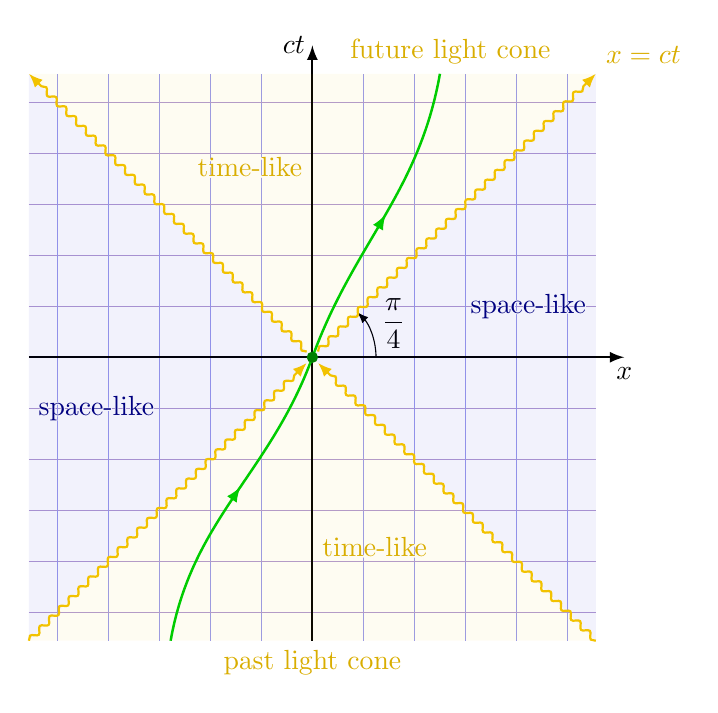
\begin{tikzpicture}[scale=1.8]
  \message{Light cone^^J}
  
  \def\xmax{2}
  \def\xmaxp{2.2} % maximum of rotated axis
  \def\Nlines{5} % number of world lines (at constant x/t)
  \pgfmathsetmacro\d{0.9*\xmax/\Nlines} % grid size
  \pgfmathsetmacro\ang{atan(1/3)} % angle between x and x' axes
  \pgfmathsetmacro\D{2*\d} 
  \coordinate (O) at (0,0);
  \coordinate (X) at (\xmax+0.2,0);
  \coordinate (T) at (0,\xmax+0.2);
  \coordinate (C) at (45:{-\D*sqrt(2)/(1-cot(\ang))});
  
  % WORLD LINE GRID
  \message{  Making world lines...^^J}
  \foreach \i [evaluate={\x=\i*\d;}] in {1,...,\Nlines}{
    \message{  Running i/N=\i/\Nlines, x=\x...^^J}
    \draw[world line]   (-\x,-\xmax) -- (-\x,\xmax);
    \draw[world line]   ( \x,-\xmax) -- ( \x,\xmax);
    \draw[world line t] (-\xmax,-\x) -- (\xmax,-\x);
    \draw[world line t] (-\xmax, \x) -- (\xmax, \x);
  }
  
  % AXES
  \draw[->,thick] (0,-\xmax) -- (T) node[left=-1] {$ct$};
  \draw[->,thick] (-\xmax,0) -- (X) node[below=0] {$x$};
 
  % LABELS
  \draw pic[->,"$\dfrac{\pi}{4}$",draw=black,angle radius=23,angle eccentricity=1.38] {angle = X--O--C};
  \node[mydarkorange,above right] at (0.1*\xmax,\xmax) {future light cone};
  \node[mydarkorange,below] at (0,-\xmax) {past light cone};
  
  % FILLS
  \fill[myblue,opacity=0.05] % SPACELIKE
    (\xmax,\xmax) -- (-\xmax,-\xmax) -- (-\xmax,\xmax) -- (\xmax,-\xmax) -- cycle;
  \fill[myorange,opacity=0.05] % TIMELIKE
    (\xmax,\xmax) -- (-\xmax,\xmax) -- (\xmax,-\xmax) -- (-\xmax,-\xmax) -- cycle;
  \node[mydarkblue,right,align=center] at (-\xmax,-0.18*\xmax)
    {\contour{myblue!5}{space-like}};
  \node[mydarkblue,left,align=center] at (\xmax,0.18*\xmax)
    {\contour{myblue!5}{space-like}};
  \node[mydarkorange,align=center] at (-0.22*\xmax,0.67*\xmax)
    {\contour{myorange!5}{time-like}};
  \node[mydarkorange,align=center] at (0.22*\xmax,-0.67*\xmax)
    {\contour{myorange!5}{time-like}};
  
  % PHOTON
  \draw[photon] ( \xmax,-\xmax) -- ( 0.02*\xmax,-0.02*\xmax);
  \draw[photon] (-\xmax,-\xmax) -- (-0.02*\xmax,-0.02*\xmax);
  \draw[photon] ( 0.02*\xmax,0.02*\xmax) -- ( \xmax,\xmax)
    node[mydarkorange,above right] {$x=ct$};
  \draw[photon] (-0.02*\xmax,0.02*\xmax) -- (-\xmax,\xmax);
  
  % PARTICLE WORLDLINE
  \draw[particle,decoration={markings,mark=at position 0.27 with {\arrow{latex}},
                                      mark=at position 0.76 with {\arrow{latex}}},postaction={decorate}]
      (-0.5*\xmax,-\xmax) to[out=80,in=-110] (O) to[out=70,in=-100] (0.45*\xmax,\xmax);
  \fill[mydarkgreen] (O) circle(0.04); % event
  
\end{tikzpicture}


\end{document}